\section{Batch and planification}

\subsection{Objectives}

	\begin{frame}
		\frametitle{Objective}
		
		Our worker is working fine, but induce too many stress on the system.We want now to deploy it as a batch.
		
		\bigskip
		As such, we want to be able to schedule it.
		
		\bigskip
		We are now going to create a batch performing the same task as our worker.
	\end{frame}

	\begin{frame}
		\frametitle{What kind use to deploy our application}
		
		\begin{center}
		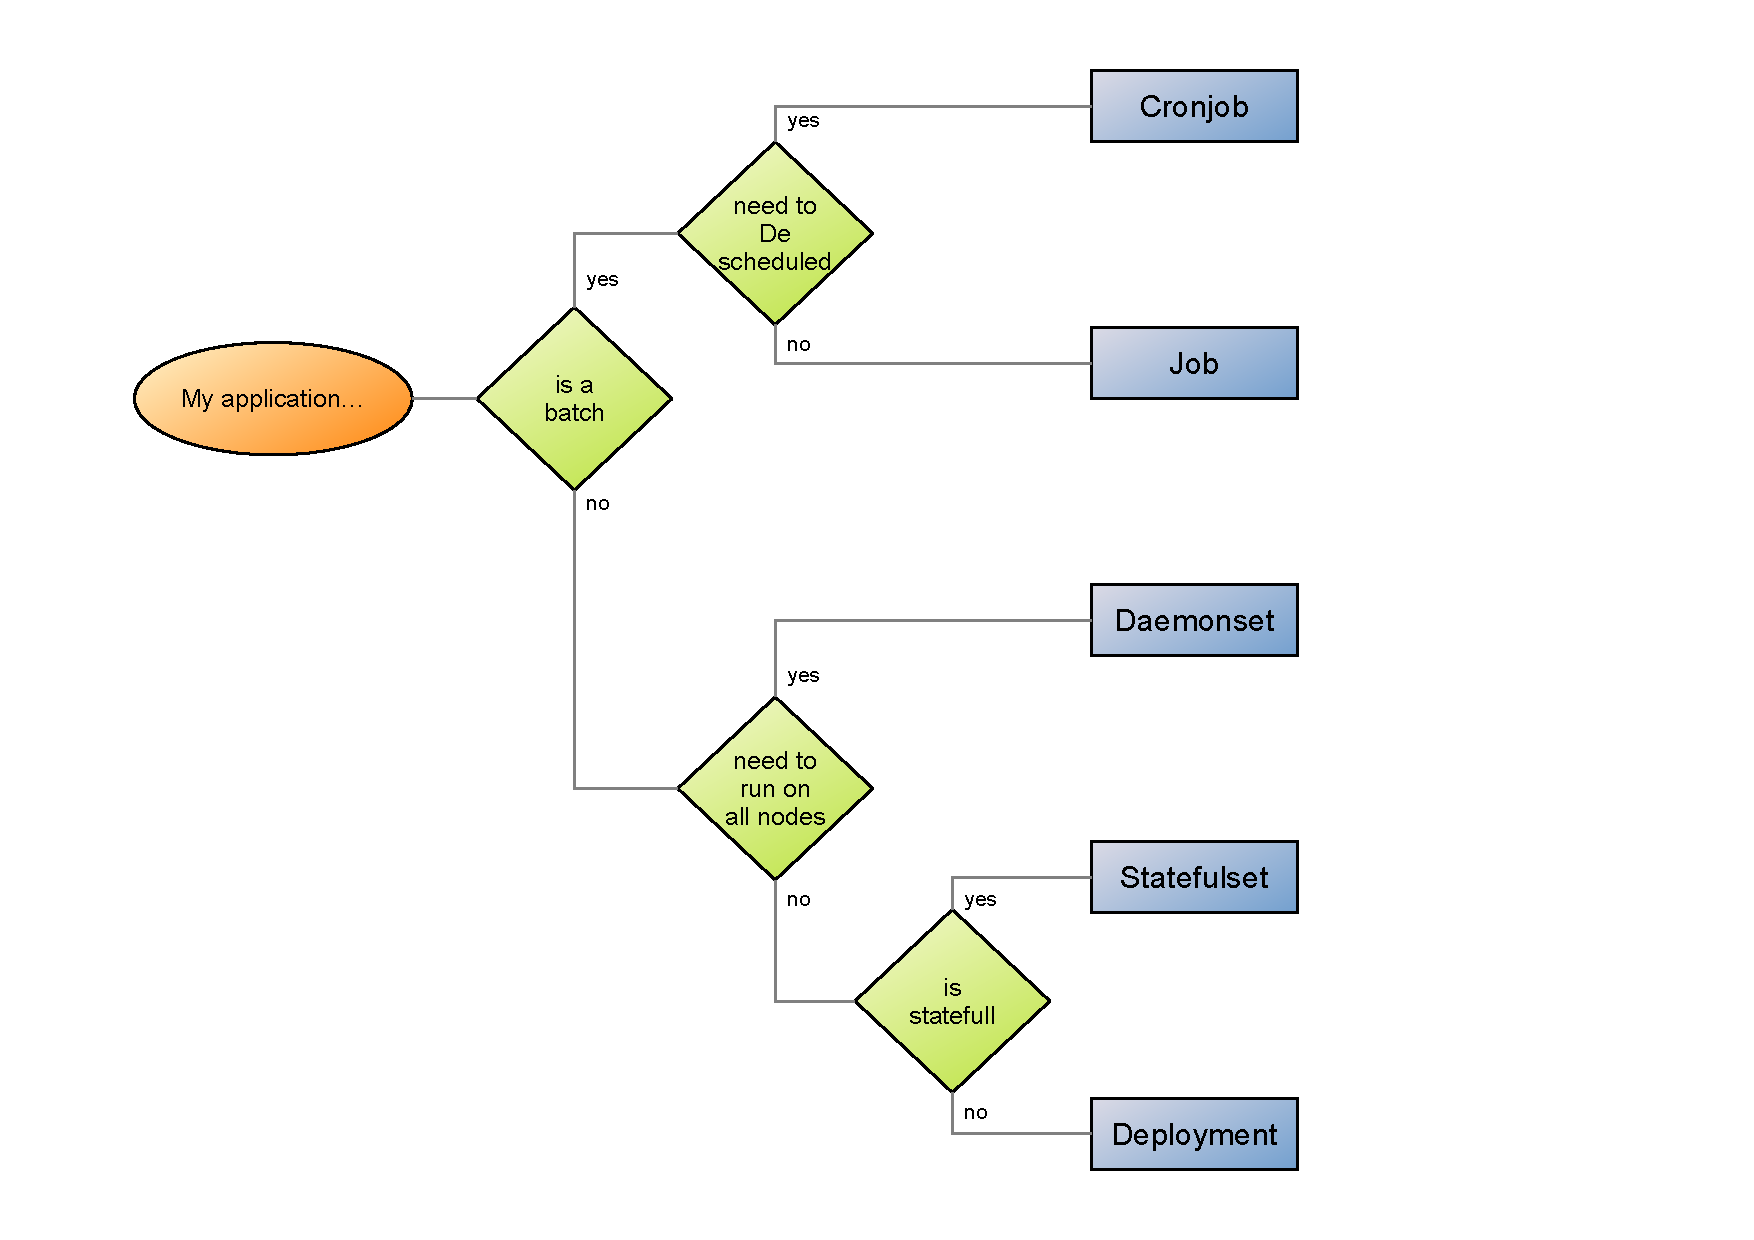
\includegraphics[height=6.8cm]{../../../resources/color/choiceDeploymentType.pdf}
		\end{center}
	\end{frame}
		
\subsection{Create a batch in kubernetes}		
		
	\begin{frame}[fragile]
		\frametitle{Create the batch}
		
		Beside the folder WORKER\_DIR, create a folder BATCH\_DIR.
		
		\bigskip
		Create the batch itself:
		\begin{block}{batch.sh}
			\begin{verbatim}
				echo "It is $(date) and all is well!"
			\end{verbatim}
		\end{block}
		Now, each execution is unitary.
	\end{frame}
	
	\begin{frame}[fragile]
		\frametitle{Exercise}

		Write a Dockerfile, build and push in the registry an image \verb|<registry>/training/batch-<id>:v1|
	\end{frame}

	\begin{frame}[fragile]
		\frametitle{solution}
		
		\begin{block}{Dockerfile}
			\begin{verbatim}
				FROM alpine
				
				COPY batch.sh .
				
				CMD /batch.sh
			\end{verbatim}
		\end{block}
		
		\begin{block}{Command line 1}
			\begin{verbatim}
				chmod u+x batch.yaml
				docker build -t <registry>/training/batch-<id>:v1 .
				docker push <registry>/training/batch-<id>:v1
			\end{verbatim}
		\end{block}
	\end{frame}
	
	\begin{frame}[fragile]
		\frametitle{Create our first CronJob}
		
		\begin{block}{cronjob.yaml}
			\begin{tiny}
				\begin{verbatim}
					apiVersion: batch/v1beta1
					kind: CronJob
					metadata:
					  name: my-batch
					spec:
					  schedule: "* * * * *"
					  jobTemplate:
					    spec:
					      template:
					        metadata:
					          labels:
					            tinkou: batch
					        spec:
					          containers:
					          - name: runner
					            image: <registry>/training/batch-<id>:v1
					            env:
					            - name: NAME
					              value: Mathilde
					          restartPolicy: Never
					          imagePullSecrets:
					          - name: regcred
				\end{verbatim}
			\end{tiny}
		\end{block}
	\end{frame}
	
	\begin{frame}[fragile]
		\frametitle{Create our first CronJob}
		
		\begin{block}{Command line 2}
			\begin{verbatim}
				stern -l tinkou=batch
			\end{verbatim}
		\end{block}
		
		\begin{block}{Command line 3}
			\begin{verbatim}
				watch kubectl get all
			\end{verbatim}
		\end{block}
		
		\begin{block}{Command line 1}
			\begin{verbatim}
				kubectl apply -f cronjob.yaml
			\end{verbatim}
			Wait for a few batches to run…
			\begin{verbatim}
				kubectl logs -l tinkou=batch
			\end{verbatim}
		\end{block}
	\end{frame}

	\begin{frame}
		\frametitle{Conclusions}
		
		\begin{block}{Conclusions}
			\begin{itemize}
				\item[$\bullet$] CronJob are easy to defined
				\item[$\bullet$] stern is less adapt than a standard kubectl logs for jobs
			\end{itemize}
		\end{block}
		
		\begin{block}{CronJobs usefull options}
			\begin{itemize}
				\item[$\bullet$] A field .spec.suspend enable to suspend the scheduling of a CronJob
				\item[$\bullet$] Jobs in error aren't removed
				\item[$\bullet$] The history limit of successfull jobs can be set
			\end{itemize}
		
		\end{block}
	\end{frame}
	
\subsection{Use a layer based configuration}	
	
	\begin{frame}
		\frametitle{Exercise}
		
		Modify the configuration to use kustomize and skaffold.
	\end{frame}
	
	\begin{frame}[fragile]
		\frametitle{A solution}
		
		\begin{block}{In a new folder configuration}
			\begin{small}
				\begin{verbatim}
					configuration
					|- base
					|  |- conf.env
					|  |- cronjob.yaml
					|  |- kustomization.yaml
					|- skaffold
					   |- conf.yaml
					   |- cronjob.yaml
					   |- kustomization.yaml
				\end{verbatim}
			\end{small}
		\end{block}

		\begin{block}{configuration/base/conf.env}
			\begin{small}
				\begin{verbatim}
					NAME=Elodie
				\end{verbatim}
			\end{small}
		\end{block}

	\end{frame}
	
	\begin{frame}[fragile]
		\frametitle{A solution}
				
		\begin{block}{configuration/base/cronjob.yaml}
			\begin{tiny}
				\begin{verbatim}
					apiVersion: batch/v1beta1
					kind: CronJob
					metadata:
					  name: my-batch
					spec:
					  schedule: "* 5 * * *"
					  jobTemplate:
					    spec:
					      template:
					        metadata:
					          labels:
					            tinkou: batch
					        spec:
					          containers:
					          - name: runner
					            image: <registry>/training/batch-<id>:v1
					            imagePullPolicy: IfNotPresent 
					            envFrom:
					            - configMapRef:
					                name: batch
					          restartPolicy: Never
				\end{verbatim}
			\end{tiny}
		\end{block}
	\end{frame}
	
	\begin{frame}[fragile]
		\frametitle{A solution}

		\begin{block}{configuration/base/kustomization.yaml creation}
			\begin{verbatim}
				touch kustomization.yaml
				kustomize edit add resource cronjob.yaml
				kustomize edit add configmap batch \
				                             --from-env-file conf.env
			\end{verbatim}
		\end{block}
	\end{frame}
	
	\begin{frame}[fragile]
		\frametitle{A solution}
		
		\begin{block}{configuration/skaffold/conf.yaml}
			\begin{verbatim}
				apiVersion: v1
				kind: ConfigMap
				metadata:
				  name: batch
				data:
				  NAME: Marina
			\end{verbatim}
		\end{block}
	\end{frame}
	
	\begin{frame}[fragile]
		\frametitle{A solution}
		
		\begin{block}{configuration/skaffold/cronjob.yaml}
		\begin{tiny}
				\begin{verbatim}
					apiVersion: batch/v1beta1
					kind: CronJob
					metadata:
					  name: my-batch
					spec:
					  schedule: "* * * * *"
					  jobTemplate:
					    spec:
					      template:
					        spec:
					          containers:
					          - name: runner
					            image: <registry>/training-<id>
					          imagePullSecrets:
					          - name: regcred
				\end{verbatim}
			\end{tiny}
		\end{block}
	\end{frame}
	
	\begin{frame}[fragile]
		\frametitle{A solution}
		
		\begin{block}{configuration/skaffold/kustomization.yaml creation}
			\begin{verbatim}
				touch kustomization.yaml
				kustomize edit fix
				kustomize edit add resource ../base
				kustomize edit add patch conf.yaml cronjob.yaml
			\end{verbatim}
		\end{block}
	\end{frame}
	
	\begin{frame}[fragile]
		\frametitle{A solution}
		
		\begin{block}{\$WORKER\_DIR/skaffold.yaml}
			\begin{verbatim}
				apiVersion: skaffold/v1beta12
				kind: Config
				build:
				  artifacts:
				  - image: <registry>/training/batch-<id>
				deploy:
				  kustomize:
				    path: configuration/skaffold
			\end{verbatim}
		\end{block}
	\end{frame}